\documentclass[footheight=20pt, footsepline, headheight=20pt, headsepline]{scrartcl}
%
\usepackage[utf8]{inputenc} % below are various important packages
\usepackage{lmodern}
\usepackage[T1]{fontenc}
\usepackage[english]{babel}
\usepackage{textcomp} 
\usepackage{amsmath}
\usepackage{mathrsfs}
\usepackage{listings}
\usepackage{latexsym}
\usepackage{amssymb}	
\usepackage{amsfonts}
\usepackage{float}
\usepackage{theorem}
\usepackage{graphicx}
\usepackage{placeins}
\usepackage{scrlayer-scrpage}
\usepackage{xcolor}
\usepackage{setspace}
\usepackage{framed}
\usepackage{hyperref} 
\usepackage{pgf,tikz,pgfplots} % possibility to insert geogebra graphs
\usepackage{mathrsfs}
\pgfplotsset{compat=1.15}\usetikzlibrary{arrows} % part of geogebra package
\usepackage{qrcode} % insert qr codes
\usepackage{multicol}
\usepackage{multirow}
\usepackage{xurl}
\usepackage{tabularx}
\usepackage{enumitem}
\usepackage{float}
\usepackage{colortbl,rotating,booktabs} % required packages for Excel2Latex


% Add to length for wider margins
\addtolength{\textwidth}{3cm} % right to margin
\addtolength{\hoffset}{-1.6cm} % left to margin
\addtolength{\voffset}{-2cm} % to top
\addtolength{\textheight}{6.5cm} % to bottom

% Headers-Footers
\definecolor{gro}{gray}{0.6} % define color
\setkomafont{pagehead}{\normalfont\sffamily} % define header
\setkomafont{pagefoot}{\normalfont\sffamily} % define footer
\addtokomafont{headsepline}{\color{gro}} % define header horizontal line



\renewcommand{\familydefault}{\sfdefault} % font
\linespread{1.2} % increase line spacing
%---------------------------------------------------------------------------
\begin{document} % every document starts with \begin{document}
%\doublespacing
\title{LAB REPORT (Lab-3) \\[1cm] \large{\textbf{CSE 3113: Microprocessor and Assembly Language Lab}}\\[1cm]} 
\author{Jahir Sadik Monon \\ Roll - 32}
\date{\vspace{10cm}  Submitted to, \\[0.1cm] Dr. Upama Kabir \\[0.5cm] Department of Computer Science and Engineering \\[0.5cm] University Of Dhaka}
\maketitle
\newpage
\tableofcontents 
%---------------------------------------------------------------------------
\newpage
\section*{Peripheral Clock Configuration (Task I)}
\addcontentsline{toc}{section}{Peripheral Clock Configuration (Task I)}
\subsection*{Clock registers of Nucleo-STM32F446RE \& their respective purpose}
\addcontentsline{toc}{subsection}{Clock registers of Nucleo-STM32F446RE \& their respective purpose}

\begin{enumerate}
    \item \textbf{RCC clock control register (RCC\_CR)}
    \\ The clock control register RCC\_CR will be used to enable and select the clock source. We can toggle the enable bits to enable PLLSAI, PLLI2S, Main PLL, HSE clock bypass, HSE clock, IHS clock and lock/unlock various ready flags.
    \item \textbf{RCC PLL configuration register (RCC\_PLLCFGR)}
    \\ This register is used to configure the PLL clock outputs according to the formulas.
        \begin{itemize}
            \item f\textsubscript{(VCO clock)} = f\textsubscript{(PLL clock input)} × (PLLN / PLLM)
            \item f\textsubscript{(PLL general clock output)} = f\textsubscript{(VCO clock)} / PLLP
            \item f\textsubscript{(USB OTG FS, SDIO)} = f\textsubscript{(VCO clock)} / PLLQ
        \end{itemize}
    \item \textbf{RCC clock configuration register (RCC\_CFGR)}
    \\  Clock configuration register RCC\_CFGR is used to configure the final bus frequencies. 
    \item\textbf{RCC clock interrupt register (RCC\_CIR)}
    \\ This register is used to configure/enable interrupt flags. We can set the interrupt flags by toggling the corresponding bits to clear/not cleared.
    \item\textbf{RCC AHB1 peripheral reset register (RCC\_AHB1RSTR)}
    \\ The Peripheral Reset Registers should cause the AHB1 peripheral's entire register set and internal state to be reset to it's power-on defaults. This means not just the registers that are exposed to the user, but also any internal registers, counters, or flags should be set as they would be when the device is initially powered on.
    \item\textbf{RCC AHB2 peripheral reset register (RCC\_AHB2RSTR)}
    \\ Just like the prior description of the AHB1 reset register, this reset register is used to cause the state of entire register set and internal state to be reset to it's power-on defaults.
    \item\textbf{RCC AHB3 peripheral reset register (RCC\_AHB3RSTR)}    
    \\ Just like the prior description of the AHB1 reset register, this reset register is used to cause the state of entire register set and internal state to be reset to it's power-on defaults.
    \item\textbf{RCC APB1 peripheral reset register (RCC\_APB1RSTR)}
    \\ Just like the prior description of the AHB1 reset register, this reset register is used to cause the state of entire register set and internal state to be reset to it's power-on defaults.
    \item\textbf{RCC APB2 peripheral reset register (RCC\_APB2RSTR)}
    \\ Just like the prior description of the AHB1 reset register, this reset register is used to cause the state of entire register set and internal state to be reset to it's power-on defaults.
    \item \textbf{RCC AHB1 peripheral clock enable register (RCC\_AHB1ENR) }
    \\ Used to enable and disable bits to control the clocks for various GPIO ports associated with AHB1.
    \item \textbf{RCC AHB2 peripheral clock enable register (RCC\_AHB2ENR) }
    \\ Used to enable and disable bits to control the clocks for various GPIO ports associated with AHB2.
    \item \textbf{RCC AHB3 peripheral clock enable register (RCC\_AHB3ENR) }
    \\ Used to enable and disable bits to control the clocks for various GPIO ports associated with AHB3.
    \item \textbf{RCC APB1 peripheral clock enable register (RCC\_APB1ENR) }
    \\ Used to enable and disable bits to control the clocks for various GPIO ports associated with APB1.
    \item \textbf{RCC APB2 peripheral clock enable register (RCC\_APB2ENR) }
    \\ Used to enable and disable bits to control the clocks for various GPIO ports associated with APB2.
    \item \textbf{RCC AHB1 peripheral clock enable in low power mode register (RCC\_AHB1LPENR)}
    \\ Used to enable or disable the AHB1 peripheral clock during Low Power (Sleep) mode.
    \item \textbf{RCC AHB2 peripheral clock enable in low power mode register (RCC\_AHB2LPENR)}
    \\ Used to enable or disable the AHB2 peripheral clock during Low Power (Sleep) mode.
    \item \textbf{RCC AHB3 peripheral clock enable in low power mode register (RCC\_AHB3LPENR)}
    \\ Used to enable or disable the AHB3 peripheral clock during Low Power (Sleep) mode.
    \item \textbf{RCC APB1 peripheral clock enable in low power mode register (RCC\_APB1LPENR)}
    \\ Used to enable or disable the APB1 peripheral clock during Low Power (Sleep) mode.
    \item \textbf{RCC APB2 peripheral clock enable in low power mode register (RCC\_APB2LPENR)}
    \\ Used to enable or disable the APB2 peripheral clock during Low Power (Sleep) mode.
    \item \textbf{RCC Backup domain control register (RCC\_BDCR)}
        \\ This register is for performing a backup domain reset, handling the real-time clock and the LSE clock.
    \item \textbf{RCC clock control \& status register (RCC\_CSR)}
        \\ This register is mainly used by the hardware to set flags after various resets occur. Software may write to the RMVF bit to clear all reset bits set by hardware.
    \item \textbf{RCC spread spectrum clock generation register (RC\_SSCGR)}
        \\ This register is used for spread spectrum clock generation for the main PLL. It has to be written to before the main PLL is enabled or after the main PLL is disabled.
    \item \textbf{RCC PLLI2S configuration register (RCC\_PLLI2SCFGR)}
        \\ This register is used to configure the PLLI2S clock outputs according to the formulas:
        \begin{itemize}
            \item f\textsubscript{(VCO clock)} = f\textsubscript{(PLLI2S clock input)} × (PLLI2SN / PLLI2SM)
            \item f\textsubscript{(PLL I2S clock output)} = f\textsubscript{(VCO clock)} / PLLI2SR
            \item f\textsubscript{(PLL SPDIFRX clock output)} = f\textsubscript{(VCO clock)} / PLLI2SP
        \end{itemize}
    \item \textbf{RCC PLL configuration register (RCC\_PLLSAICFGR)}
        \\ This register is used to configure the PLLSAI clock outputs according to the formulas:
        \begin{itemize}
            \item f\textsubscript{(VCO clock)} = f\textsubscript{(PLLSAI clock input)} × (PLLSAIN / PLLM)
            \item f\textsubscript{(PLL SAI 48MHz clock output)} = f\textsubscript{(VCO clock)} / PLLSAIP
            \item f\textsubscript{(PLL SAI1 clock output)} = f\textsubscript{(VCO clock)} / PLLSAIQ
        \end{itemize}
    \item \textbf{RCC Dedicated Clock Configuration Register (RCC\_DCKCFGR)}
        \\ This register allows to configure the timer clock prescalers and the PLLSAI and PLLI2S output clock dividers for SAIs peripherals according to the following formula:
        \begin{itemize}
            \item f\textsubscript{(PLLSAIDIVQ clock output)} = f\textsubscript{(PLLSAI\_Q)} / PLLSAIDIVQ
            \item f\textsubscript{(PLLI2SDIVQ clock output)} = f\textsubscript{(PLLI2S\_Q)} / PLLI2SDIVQ
        \end{itemize}
    \item \textbf{RCC clocks gated enable register (CKGATENR)}
        \\ This register allows to enable or disable the clock gating for the specified IPs.
    \item \textbf{RCC dedicated clocks configuration register 2 (DCKCFGR2)}
        \\ This register allows to enable or disable the clock gating for the specified IPs.
\end{enumerate}

\subsection*{List of memory addresses of the Clock registers}
\addcontentsline{toc}{subsection}{List of memory addresses of the Clock registers}
\vspace{0.5cm}
\begin{tabular}{ |c|c| }
    \hline
    \textbf{Register Name} & \textbf{Memory Address}  \\
    \hline
    RCC clock control register (RCC\_CR) & 40023800\\
    \hline
    RCC PLL configuration register (RCC\_PLLCFGR) & 40023804\\
    \hline
    RCC clock configuration register (RCC\_CFGR) & 40023808\\
    \hline
    RCC clock interrupt register (RCC\_CIR) & 4002380C\\
    \hline
    RCC AHB1 peripheral reset register (RCC\_AHB1RSTR) & 40023810\\
    \hline
    RCC AHB2 peripheral reset register (RCC\_AHB2RSTR) & 40023814\\
    \hline
    RCC AHB3 peripheral reset register (RCC\_AHB3RSTR) & 40023818\\
    \hline
    RCC APB1 peripheral reset register (RCC\_APB1RSTR) & 40023820\\
    \hline
    RCC APB2 peripheral reset register (RCC\_APB2RSTR) & 40023824\\
    \hline
    RCC AHB1 peripheral clock enable register (RCC\_AHB1ENR)  & 40023830\\
    \hline
    RCC AHB2 peripheral clock enable register (RCC\_AHB2ENR) & 40023834\\
    \hline
    RCC AHB3 peripheral clock enable register (RCC\_AHB3ENR) & 40023838\\
    \hline
    RCC APB1 peripheral clock enable register (RCC\_APB1ENR) & 40023840\\
    \hline
    RCC APB2 peripheral clock enable register (RCC\_APB2ENR) & 40023844\\
    \hline
    RCC AHB1 peripheral clock enable in low power mode register (RCC\_AHB1LPENR) & 40023850\\
    \hline
    RCC AHB2 peripheral clock enable in low power mode register (RCC\_AHB2LPENR) & 40023854\\
    \hline
    RCC AHB3 peripheral clock enable in low power mode register (RCC\_AHB3LPENR) & 40023858\\
    \hline
    RCC APB1 peripheral clock enable in low power mode register (RCC\_APB1LPENR) & 40023860\\
    \hline
    RCC APB2 peripheral clock enable in low power mode register (RCC\_APB2LPENR) & 40023864\\
    \hline
    RCC Backup domain control register (RCC\_BDCR) & 40023870\\
    \hline
    RCC clock control \& status register (RCC\_CSR) & 40023874\\
    \hline
    RCC spread spectrum clock generation register (RC\_SSCGR) & 40023880\\
    \hline
    RCC PLLI2S configuration register (RCC\_PLLI2SCFGR) &  40023884\\
    \hline
    RCC PLL configuration register (RCC\_PLLSAICFGR) & 40023888\\
    \hline
    RCC Dedicated Clock Configuration Register (RCC\_DCKCFGR) & 4002388C\\
    \hline
    RCC clocks gated enable register (CKGATENR) & 40023890\\
    \hline
    RCC dedicated clocks configuration register 2 (DCKCFGR2) & 40023894\\
    \hline
\end{tabular}
\vspace{.5cm}
\section*{General Purpose Input/ Output Registers (Task II)}
\addcontentsline{toc}{section}{General Purpose Input/Output Registers (Task II)}
\subsection*{GPIO register of Nucleo-STM32F446RE \& their respective purpose}
\addcontentsline{toc}{subsection}{GPIO register of Nucleo-STM32F446RE \& their respective purpose}
\begin{enumerate}
    \item \textbf{GPIO port mode register (GPIOx\_MODER)}, where x is between A to H.
    \par These bits are written by software to configure the I/O direction mode. These modes are: Input mode, General purpose output mode, Alternative function mode, Analog mode.
    \item \textbf{GPIO port output type register (GPIOx\_OTYPER)}, where x is between A to H.
    \par These bits are written by software to configure the output type of the I/O port.
    \item \textbf{GPIO port output speed register (GPIOx\_OSPEEDR)}, where x is between A to H.
    \par These bits are written by software to configure the I/O output speed. The slew rate, or the pace at which a signal can vary from low to high values (the "rise time" and "fall time"), is controlled by the GPIO speed register. We can increase the rate of change of the output voltage by increasing the GPIO speed (reducing rise time). However, when the GPIO speed grows, so does the circuit's power consumption and noise output. Unless there is a compelling reason to increase GPIO speed, we keep it modest by default.
    \item \textbf{GPIO port pull-up/pull-down register (GPIOx\_PUPDR)}, where x is between A to H.
    \par These bits are written by software to configure the I/O pull-up or pull-down.
    
    \item \textbf{GPIO port input data register (GPIOx\_IDR)}, where x is between A to H.
    \\ These bits are read-only and can be accessed in word mode only. They contain the input value of the corresponding I/O port.
    \item \textbf{GPIO port output data register (GPIOx\_ODR)}, where x is between A to H.
    \\ These bits can be read and written by software. For atomic bit set/reset, the ODR bits can be individually set and reset by writing to the GPIOx\_BSRR register (x = A..H).
   \\ We can configure the output value of the port using this register. This is used when we want to output a word.
   \item \textbf{GPIO port bit set/reset register (GPIOx\_BSRR)}, where x is between A to H.
   \\These bits are write-only and can be accessed in word, half-word or byte mode. A read to these bits returns the value 0x0000. 
   \\This and the GPIO port output data register (GPIOx\_ODR) essentially does the same job. But in GPIOx\_ODR, we can write the output word on it, and it will be sent. But the GPIOx\_BSRR register is for more atomic control of the same thing.
   
   \item \textbf{GPIO port configuration lock register (GPIOx\_LCKR)}, where x is between A to H.
    \\ This register is used to lock the configuration of the port bits when a correct write sequence is applied to bit 16 (LCKK). The value of bits [15:0] is used to lock the configuration of the GPIO.
    \item \textbf{GPIO alternate function low register (GPIOx\_AFRL)}, where x is between A to H.
    \\ These bits are written by software to configure alternate function I/Os
    \item \textbf{GPIO alternate function high register (GPIOx\_AFRH)}, where x is between A to H.
    \\ These bits are written by software to configure alternate function I/Os

\end{enumerate}
\subsection*{List of memory addresses of the GPIO registers}
\addcontentsline{toc}{subsection}{List the memory addresses of the GPIO registers}
\vspace{.5cm}


\begin{center}
\begin{tabular}{||c c c||} 
 \hline
 Peripheral & From & To \\ [0.5ex] 
 \hline\hline
 GPIOH & 0x40021C00 & 0x40021FFF\\ 
 \hline
 GPIOG & 0x40021800 & 0x40021BFF\\
 \hline
 GPIOF & 0x40021400 & 0x400217FF\\
 \hline
 GPIOE & 0x40021000 & 0x400213FF\\
 \hline
 GPIOD & 0X40020C00 & 0x40020FFF\\
  \hline
 GPIOC & 0x40020800 & 0x40020BFF\\
  \hline
 GPIOB & 0x40020400 & 0x400207FF\\
  \hline
 GPIOA & 0x40020000 & 0x400203FF\\ [1ex] 
 \hline
\end{tabular}
\end{center}


%----------------------------------------------------------------------------------
\newpage
\FloatBarrier
\section*{Task III}
\addcontentsline{toc}{section}{Task III}
\subsection*{Problem Statement}
\addcontentsline{toc}{subsection}{Problem Statement}
Write an assembly language to perform all the logical operations (AND,OR,NOR,NAND,XOR,XNOR) on two 16-bit variables. Repeat it for two 32-bit variables.
\subsection*{Detail explanation of the code}
\addcontentsline{toc}{subsection}{Detail explanation of the code}
\textbf{Logical operations on two 16 bit numbers:}\\
First I stored two arbitrary 16-bit integers 11 and 7 on register \$r7 \& \$r6 using \verb |MOVW| operation, which restricts the input to 16-bit immediate operands. I have shown the result of logical operations using registers \$r5 to \$r0. AND, OR, and XOR logical operations have direct instructions in ARM, so the operations are as simple as,\\
\verb |AND r5, r6, r7|\\
\verb|ORR r4, r6, r7|\\
\verb|EOR r1, r6, r7|\\
The other three operations are negation of these three. We calculate negation by XORing the register value found after the AND, OR, and XOR operations with 32 1-bits (4294967295 in decimal). For example, \\
\verb|NAND = (Result of AND) XOR (4294967295)|\\
Finally, as the operations are done on 16-bit numbers, we loaded upper immediate 16 bits with 1's for NOR, NAND, XNOR, whereas for AND, OR, XOR it wasn't necessary.\\
\textbf{Logical operations on two 32 bit numbers:}\\
First I stored two arbitrary 32-bit integers 4289724416 and 4291821568 on register \$r7 \& \$r6 using \verb |MOV32| operation, which loads 32-bit immediate operands. I have shown the result of logical operations using registers \$r5 to \$r0. AND, OR, and XOR logical operations have direct instructions in ARM, so the operations are as simple as,\\
\verb |AND r5, r6, r7|\\
\verb|ORR r4, r6, r7|\\
\verb|EOR r1, r6, r7|\\
The other three operations are negation of the result of these three instructions. We calculate the negation by XORing the register value found after the AND, OR, and XOR operations with 32 1-bits (4294967295 in decimal). For example, \\
\verb|NAND = (Result of AND) XOR (4294967295)|\\
In this case we didn't need to load upper immediate values with 0's, because we're dealing with 32 bit numbers.
\subsection*{Detail description of the instruction used to design the program}
\addcontentsline{toc}{subsection}{Detail description of the instruction used to design the program}
\textbf{AND}\\The \verb|AND| instruction performs bitwise \verb|AND| operations on the values in Rn and Operand2.\\
\verb|AND{S}{cond} Rd, Rn, Operand2|\\
\textbf{ORR}\\The \verb|ORR| instruction performs bitwise \verb|ORR| operations on the values in Rn and Operand2.\\
\verb|ORR{S}{cond} Rd, Rn, Operand2|\\
\textbf{EOR}\\The \verb|EOR| instruction performs bitwise Exclusive OR operations on the values in Rn and Operand2.\\
\verb|EOR{S}{cond} Rd, Rn, Operand2|\\
\textbf{MOVW}\\The \verb|MOVW| instruction only allows \#imm16 values to be loaded into the registers.\\
\textbf{MOVT}\\\verb|MOVT| writes \#imm16 to \verb|Rd[31:16]|, without affecting \verb|Rd[15:0]|.\\
\verb|MOVT{cond} Rd, #imm16|\\
\textbf{MOV}\\
The \verb|MOV| instruction copies the value of Operand2 into Rd.\\
\verb|MOV{S}{cond} Rd, Operand2|\\
\textbf{MOV32 pseudo-instruction}\\
\verb|MOV32| always generates two 32-bit instructions, a \verb|MOV|, \verb|MOVT| pair. This enables you to load any 32-bit immediate, or to access the whole 32-bit address space.\\
\verb|MOV32{cond} Rd, expr|

\FloatBarrier
\subsection*{Screenshot of the state of the system after the code has been loaded}
\addcontentsline{toc}{subsection}{Screenshot of the state \& status registers of the system after the code has been loaded}
\begin{figure}[ht]
    \centering
    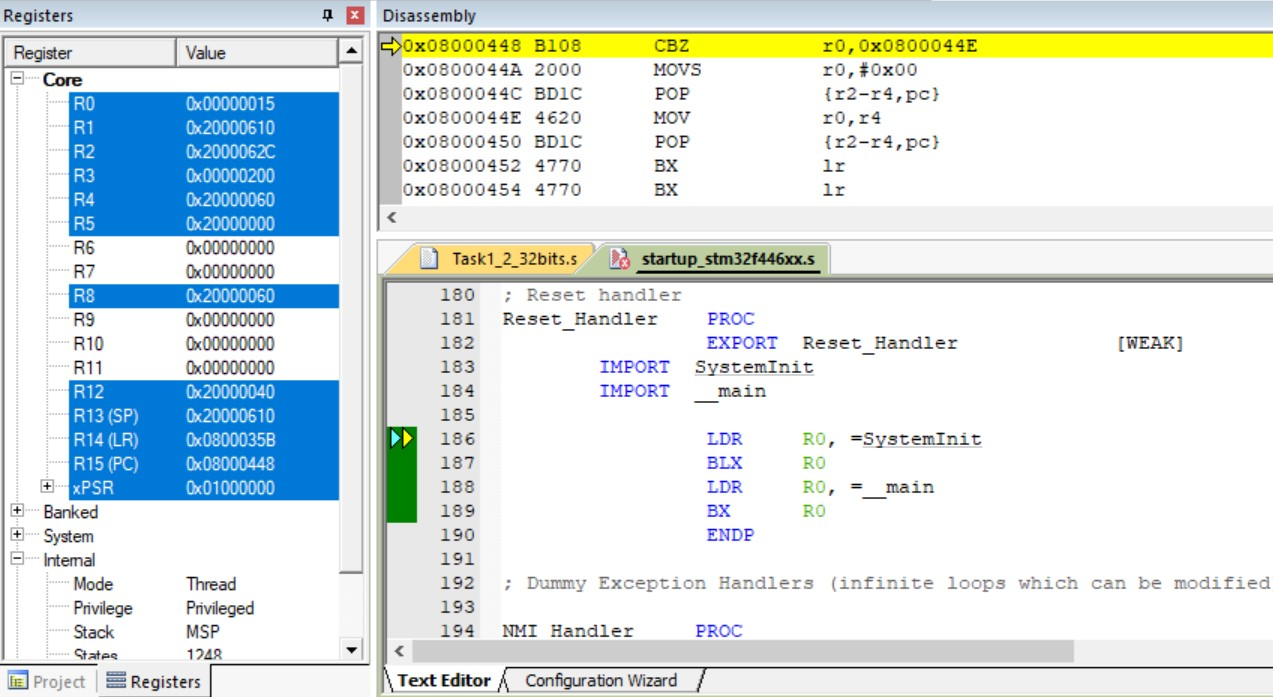
\includegraphics[scale=.7]{images/Task1_1Before1.jpg}
    \caption{After loading the code for 16-bit operands on the system (Task1.s)}
    \label{fig:before_task_one}
\end{figure}
\FloatBarrier
\begin{figure}[ht]
    \centering
    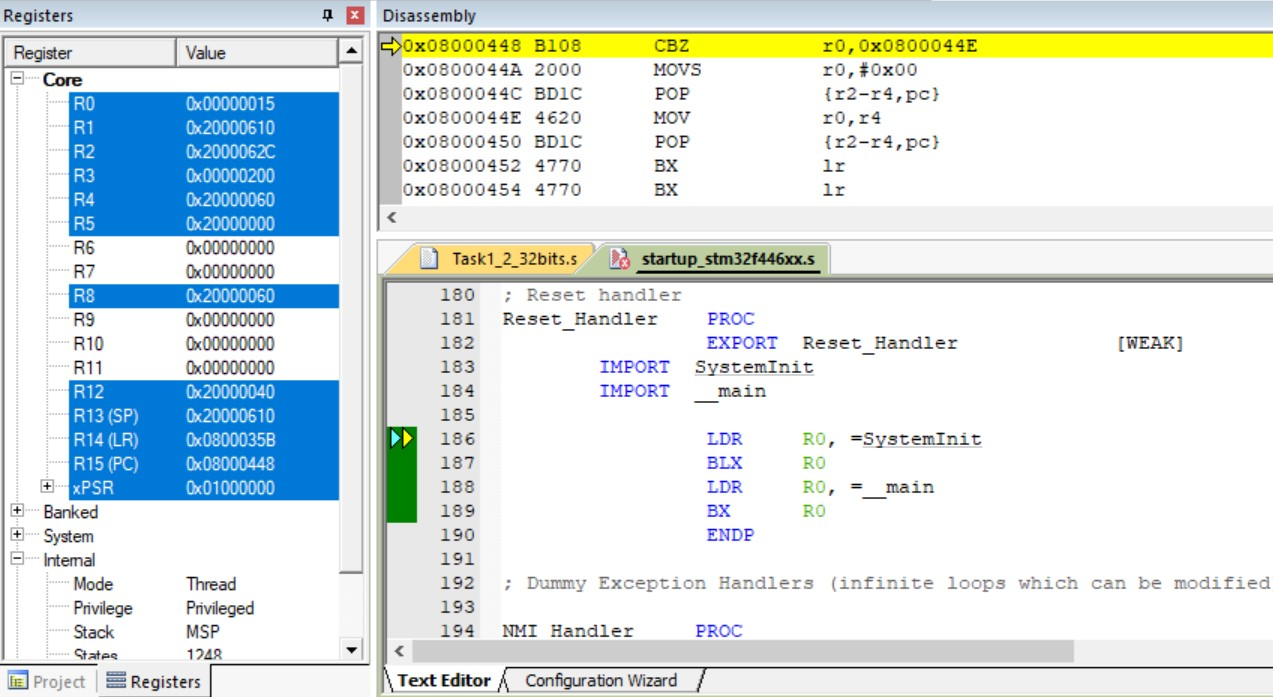
\includegraphics[scale=.7]{images/Task1_1Before1.jpg}
    \caption{After loading the code for 32-bit operands on the system (Task1\_2\_32bits.s)}
    \label{fig:before_task_one_one}
\end{figure}
\FloatBarrier
Here we can see that the registers are loaded with random values as the program is only loaded to the system and not executed yet.
\subsection*{Screenshot of the state of the system after the code has been executed}
\addcontentsline{toc}{subsection}{Screenshot of the state \& status registers of the system after the code has been executed}
\begin{figure}[h!]
    \centering
    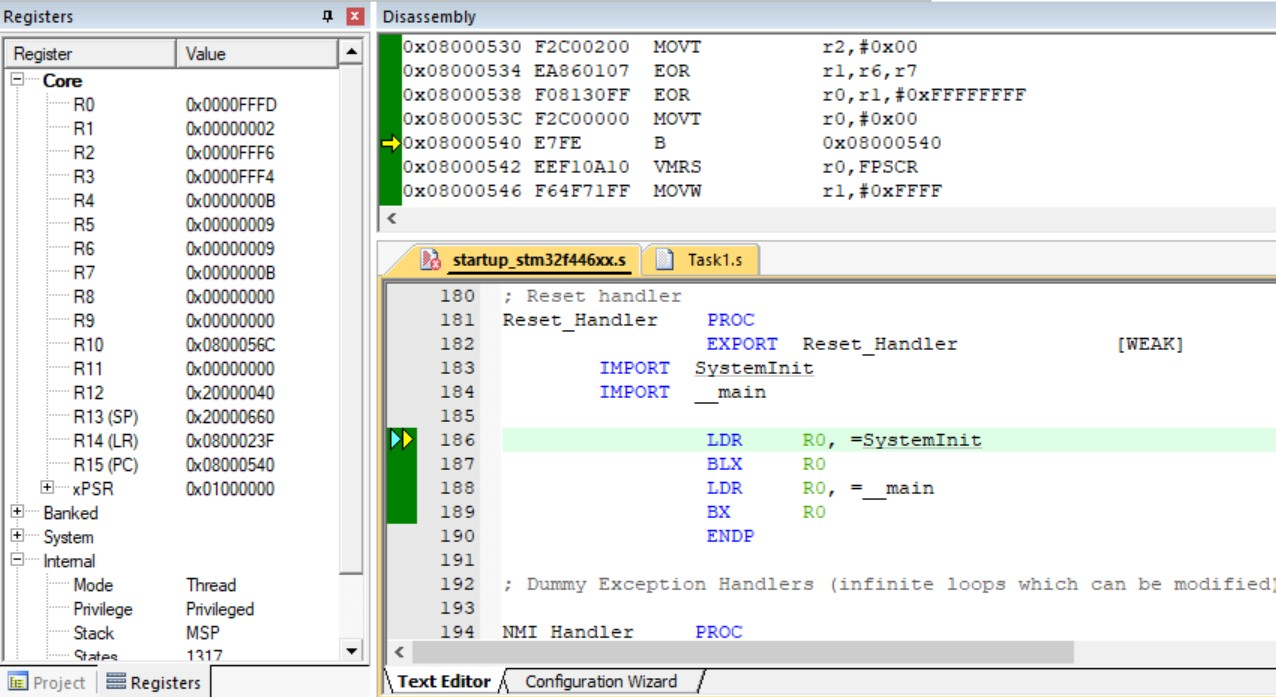
\includegraphics[scale=.7]{images/Task1After1.jpg}
    \caption{After executing the code for 16-bit operands on the system (Task1.s)}
    \label{fig:after_task_one}
\end{figure}
\FloatBarrier
As we can see from the screenshot of register values after execution of the code, the registers \$r5 to \$r0 holds the result of AND, OR, NOR, NAND, XOR and XNOR operations, in that order and the upper 16 bits are all 0's as we've restricted the input to only 16-bit values.
\begin{figure}[ht]
    \centering
    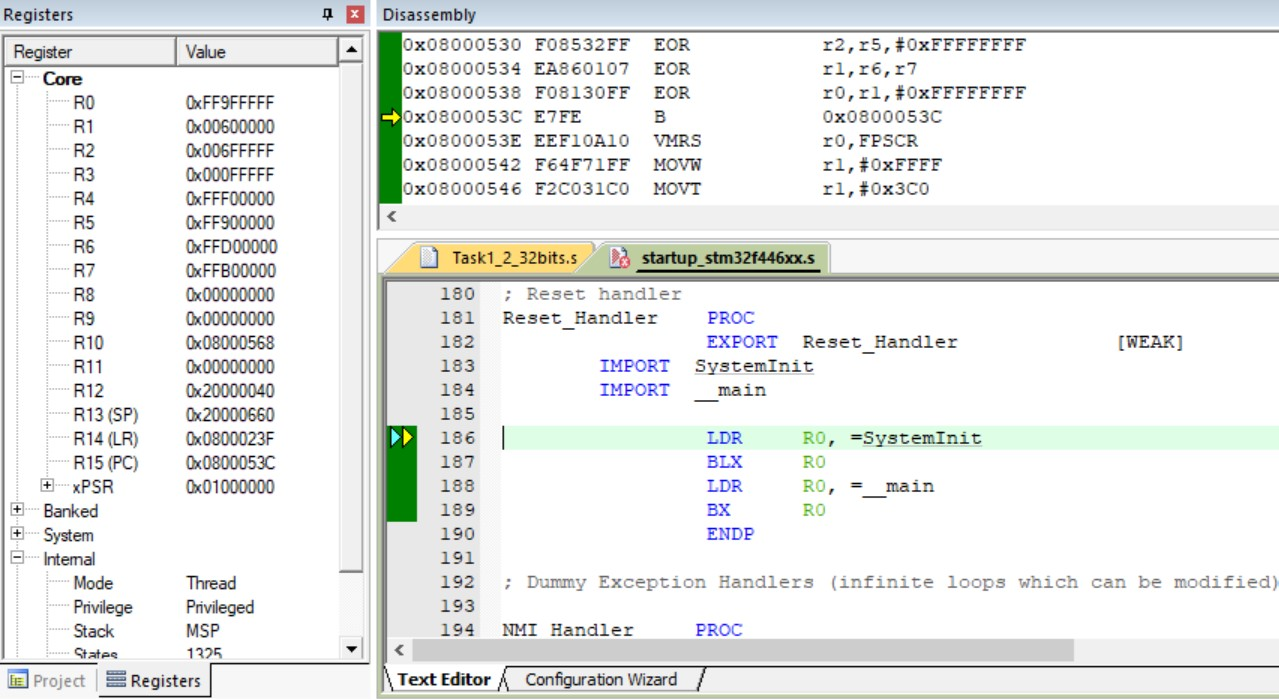
\includegraphics[scale=.7]{images/Task1_1After1.jpg}
    \caption{After executing the code for 32-bit operands on the system (Task1\_2\_32bits.s)}
    \label{fig:after_task_one_one}
\end{figure}
\FloatBarrier
As we can see from the screenshot of register values after execution of the code, the registers \$r5 to \$r0 holds the result of AND, OR, NOR, NAND, XOR and XNOR operations, in that order.

%------------------------------------------------------------------------------------
\FloatBarrier
\section*{Task IV}
\addcontentsline{toc}{section}{Task IV}
\subsection*{Problem Statement}
\addcontentsline{toc}{subsection}{Problem Statement}
Write an assembly language to perform all the shift operations (LSR, ASR, LSL) on a 32-bit variable.
\subsection*{Detail explanation of the code}
\addcontentsline{toc}{subsection}{Detail explanation of the code}
This code is simple because there are direct instructions available for LSR(Logical Shift Right), ASR(Arithmetic Shift Right), and LSL(Logical Shift Left) operations. \\I loaded the register \$r4 with an arbitrary value (4294967295) and \$r3 with shift amount of 2. Then we have found the results using, \\
\verb|LSR r2, r4, r3|\\
\verb|ASR r1, r4, r3|\\
\verb|LSL r0, r4, r3|
\subsection*{Detail description of the instruction used to design the program}
\addcontentsline{toc}{subsection}{Detail description of the instruction used to design the program}
\textbf{MOV32 pseudo-instruction}\\
\verb|MOV32| always generates two 32-bit instructions, a \verb|MOV|, \verb|MOVT| pair. This enables you to load any 32-bit immediate, or to access the whole 32-bit address space.\\
\verb|MOV32{cond} Rd, expr|\\
\textbf{LSR}\\
\verb|LSR| provides the unsigned value of a register divided by a variable power of two, inserting zeros into the vacated bit positions.\\
\verb|LSR{S}{cond} Rd, Rm, Rs|\\
\verb|LSR{S}{cond} Rd, Rm, #sh|\\
\textbf{ASR}\\
\verb|ASR| provides the signed value of the contents of a register divided by a power of two. It copies the sign bit into vacated bit positions on the left.\\
\verb|ASR{S}{cond} Rd, Rm, Rs|\\
\verb|ASR{S}{cond} Rd, Rm, #sh|\\
\textbf{LSL}\\
\verb|LSL| provides the value of a register multiplied by a power of two, inserting zeros into the vacated bit positions.\\
\verb|LSL{S}{cond} Rd, Rm, Rs|\\
\verb|LSL{S}{cond} Rd, Rm, #sh|

\FloatBarrier
\subsection*{Screenshot of the state of the system after the code has been loaded}
\addcontentsline{toc}{subsection}{Screenshot of the state \& status registers of the system after the code has been loaded}
\begin{figure}[ht]
    \centering
    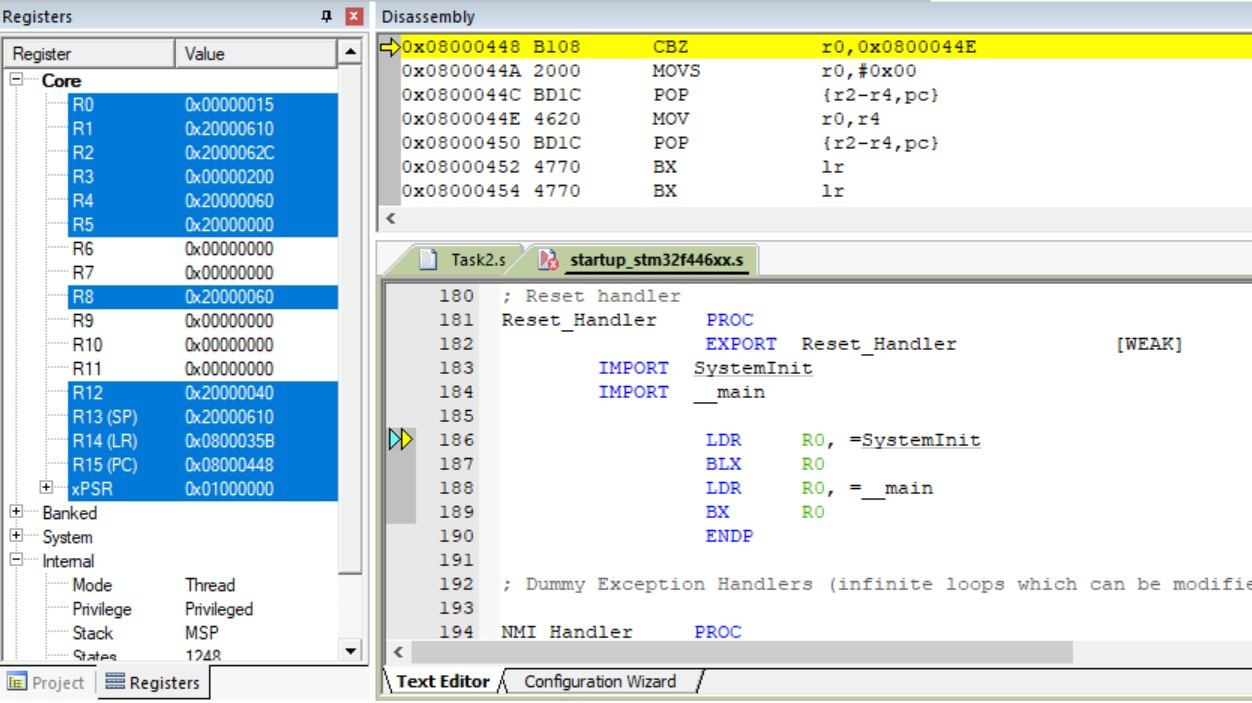
\includegraphics[scale=.7]{images/Task2Before1.jpg}
    \caption{After loading the code on the system (Task2)}
    \label{fig:before_task_two}
\end{figure}
\FloatBarrier
Here we can see that the registers are loaded with random values as the program is only loaded to the system and not executed yet.
\subsection*{Screenshot of the state of the system after the code has been executed}
\addcontentsline{toc}{subsection}{Screenshot of the state \& status registers of the system after the code has been executed}
\begin{figure}[h!]
    \centering
    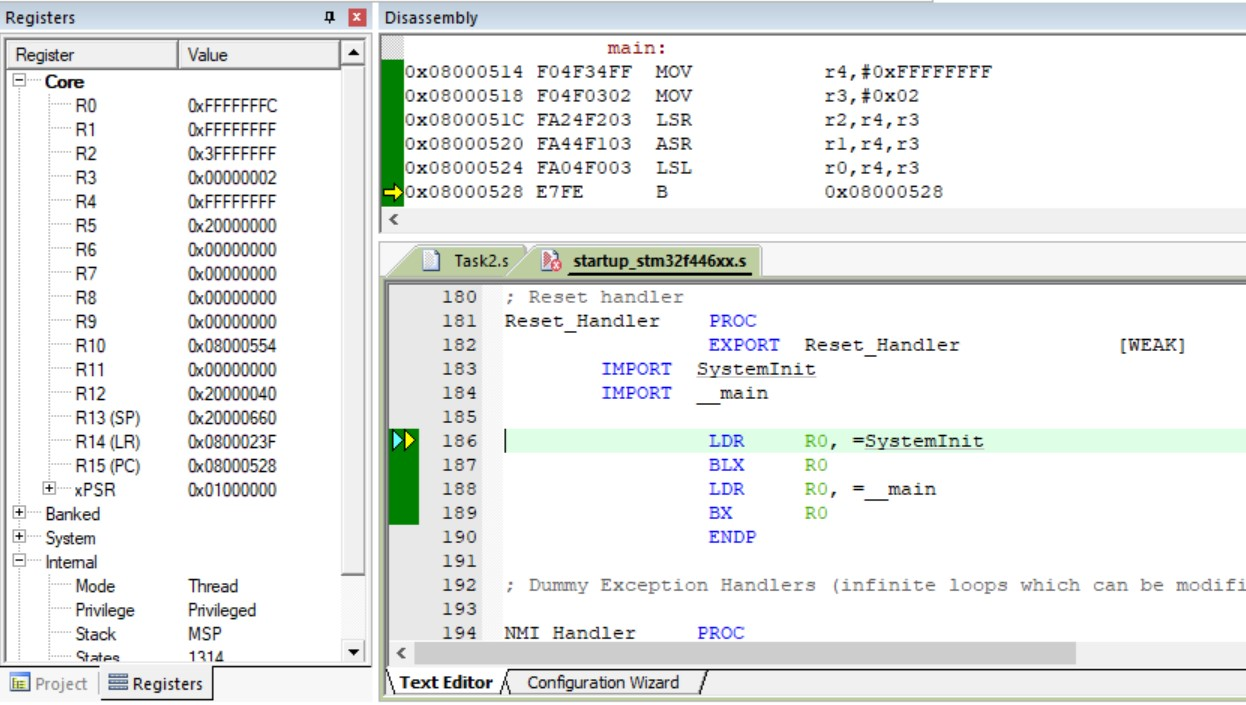
\includegraphics[scale=.7]{images/Task2After1.jpg}
    \caption{After executing the code on the system (Task2)}
    \label{fig:after_task_two}
\end{figure}
\FloatBarrier
As we can see from the screenshot of register values after execution of the code, the registers \$r2, \$r1, and \$r0 holds the result of operations LSR, ASR and LSL respectively.

%------------------------------------------------------------------------------------
\FloatBarrier
\section*{Task V}
\addcontentsline{toc}{section}{Task V}
\subsection*{Problem Statement}
\addcontentsline{toc}{subsection}{Problem Statement}
Write an assembly language to perform all the arithmetic operations (Addition, Subtraction and Multiplication) on two variables. Restrict input values to avoid overflow. Repeat the same operations to handle overflow.
\subsection*{Detail explanation of the code}
\addcontentsline{toc}{subsection}{Detail explanation of the code}
%------------------------------------------------------------------------------------
\textbf{Restricting input values to avoid overflow:}\\
The case for restricting input values, so that no overflow can occur, is simple. Because, to make sure the arithmetic addition, subtraction, and multiplication doesn't result in overflow in 32 bits, we have to restrict the inputs to only 16-bit values. The \verb |MOVW \$rn, #imm16| operation only allows 16-bit immediate values to be loaded. The rest of the code for this case is simple addition, subtraction and multiplication of values. We don't have to check the flags in this case either, because we're restricting the input, no overflow can occur.\\
\textbf{Repeating the same operations to handle overflow:}\\
The case for handling multiplication overflow is a little more complicated, as there is no in-built overflow detecting mechanism for 32-bit multiplications, as the results can be 64-bits.\\ 
Detecting overflow for addition and subtractions can easily be done using \verb|xPSR| values at runtime, which shows the runtime values of flag registers.\\ 
If overflow occurs in addition, carry flag is set. So \verb|xPSR[C] = 1|\\
If overflow occurs in subtraction, carry flag \& negative flag is set. So,  \verb|xPSR[C] = 1 & xPSR[N] = 1|\\
\textbf{Problem with detecting overflow in multiplication}\\
Like addition and subtraction, detecting overflow for multiplication cannot be done simply using flag values. \\ ARM's \verb|MUL| instruction can take the s suffix to update the flags, it only updates the n and z flags. Consider the following:\\
\verb|ldr     r0, =100000|\\
\verb|muls    r0, r0, r0|\\
It is, of course, not possible to represent \verb|100000 × 100000| in a 32-bit unsigned integer, because \verb|muls| does not report the overflow in this case. A likely explanation for this limitation is that addition and subtraction overflows (and carries) can be used to implement 64-bit arithmetic, but the same is not true for \verb|MUL| as an operation may overflow by more than one bit. Indeed, \verb|100000 × 100000| should result in \verb|10000000000|, or \verb|0x2540be400|, which cannot be reconstructed as a 64-bit quantity from the 32-bit result and the \verb|APSR| flags alone.\\
The ARM architecture does, however, provides a facility for multiplying two 32-bit quantities to produce a 64-bit result. This operation cannot overflow:\\
\verb|LDR     r0, =100000|\\
\verb|SMULL   r2, r3, r0, r0      ;   Signed: [r3:r2] = r0 * r0|\\
\verb|UMULL   r2, r3, r0, r0      ; Unsigned: [r3:r2] = r0 * r0|\\
The \verb|SMULL| and \verb|UMULL| instruction can also set the flags if I add the s suffix, but as before, this isn't terribly useful for detecting 32-bit overflow.\\
\textbf{Detecting Unsigned Overflow using} \verb|UMULL|\\
Detecting unsigned overflow using \verb|UMULL| is actually fairly trivial. Only if the multiplication overflows will the high word of the result be non-zero, so we can use the \verb|UMULL| instruction to get a 64-bit result and test the top word in a scratch register. Here, we use ip as a scratch register 1.
\begin{verbatim}
ldr     r0, =100000
umull   r0, ip, r0, r0      @   [ip:r0] = r0 * r0
cmp     ip, #0
@ ----
bne     <somewhere>   @ Branch if we overflowed.
beq     <elsewhere>   @ Branch if we did not overflow.
\end{verbatim}
So in our solution we,
\begin{itemize}
    \item Use \verb|UMULL| to multiply the two numbers and store in result registers [r3:r4] = (r8*r7).
    \item Compare upper 32 bits of result (\$r3) with zero. If it is equal to zero, then the multiplication didn't overflow. If not equal, the overflow occurred.
\end{itemize}
So in my code I did,
\begin{verbatim}
UMULL r4, r3, r8, r7	;Unsigned mult. Result regs [r3:r4] = (r8*r7)
CMP  r3, #0				;Checks if first 32 bits of previous mul is 0
MOVNE r2, #1			;If first 32 bits weren't = 0, overflow occurred
\end{verbatim}


\subsection*{Detail description of the instruction used to design the program}
\addcontentsline{toc}{subsection}{Detail description of the instruction used to design the program}
\textbf{MOV}\\
The \verb|MOV| instruction copies the value of Operand2 into Rd.\\
\verb|MOV{S}{cond} Rd, Operand2|\\
\verb|MOV{cond} Rd, #imm16|\\
\textbf{MOVW}\\The \verb|MOVW| instruction only allows \#imm16 values to be loaded into the registers.\\
\textbf{ADD}\\
The \verb|ADD| instruction adds the values in Rn and Operand2 or imm12.\\
\verb|ADD{S}{cond} Rd, Rn, Operand2|\\
\textbf{SUB}\\
The \verb|SUB| instruction subtracts the value of Operand2 or imm12 from the value in Rn.\\
\verb|SUB{S}{cond} Rd, Rn, Operand2|\\
\textbf{CMP}\\
The \verb|CMP| instruction subtracts the value of Operand2 from the value in Rn. This is the same as a \verb|SUBS| instruction, except that the result is discarded.\\
\verb|CMP{cond} Rn, Operand2|\\
\textbf{UMULL}\\
The \verb|UMULL| instruction interprets the values from Rn and Rm as unsigned integers. It multiplies these integers and places the least significant 32 bits of the result in \verb|RdLo|, and the most significant 32 bits of the result in \verb|RdHi|.\\
\verb|UMULL{S}{cond} RdLo, RdHi, Rn, Rm|\\
\textbf{MOV32 pseudo-instruction}\\
\verb|MOV32| always generates two 32-bit instructions, a \verb|MOV|, \verb|MOVT| pair. This enables you to load any 32-bit immediate, or to access the whole 32-bit address space.\\
\verb|MOV32{cond} Rd, expr|


%------------------------------------------------------------------------------------
\FloatBarrier
\subsection*{Screenshot of the state of the system after the code has been loaded}
\addcontentsline{toc}{subsection}{Screenshot of the state \& status registers of the system after the code has been loaded}
\begin{figure}[ht]
    \centering
    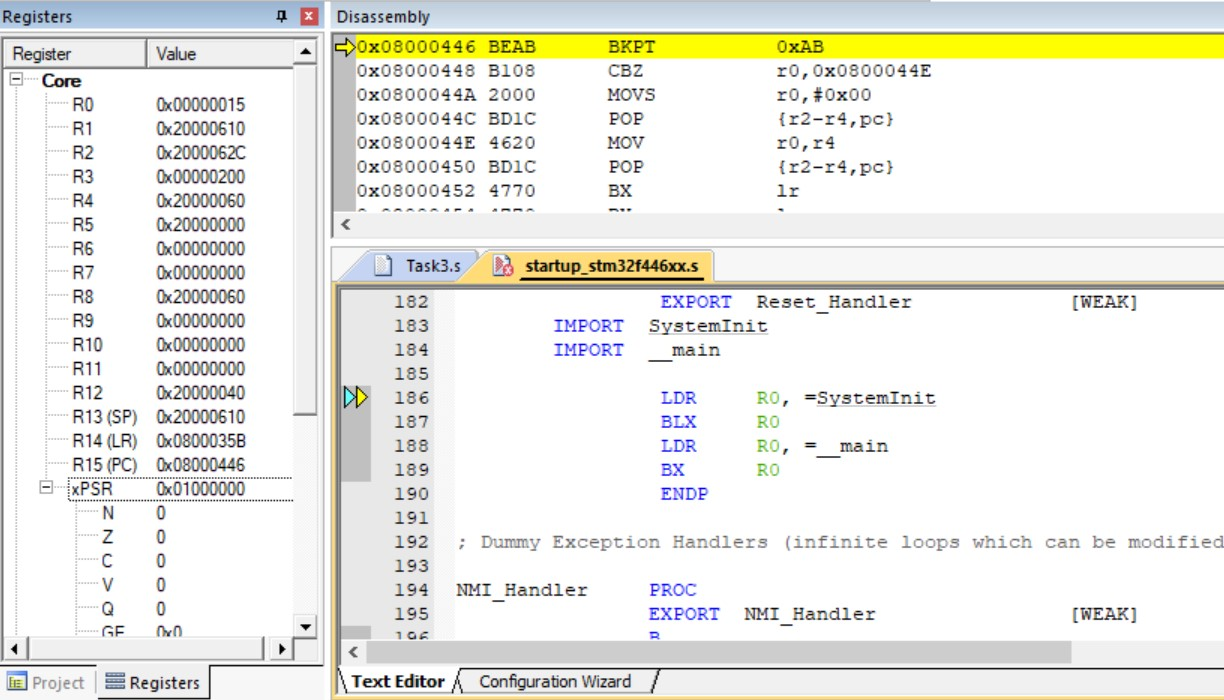
\includegraphics[scale=.7]{images/Task3_1Before1.jpg}
    \caption{After loading the code on the system (Task3)}
    \label{fig:before_task_three_one}
\end{figure}
\FloatBarrier
\begin{figure}[ht]
    \centering
    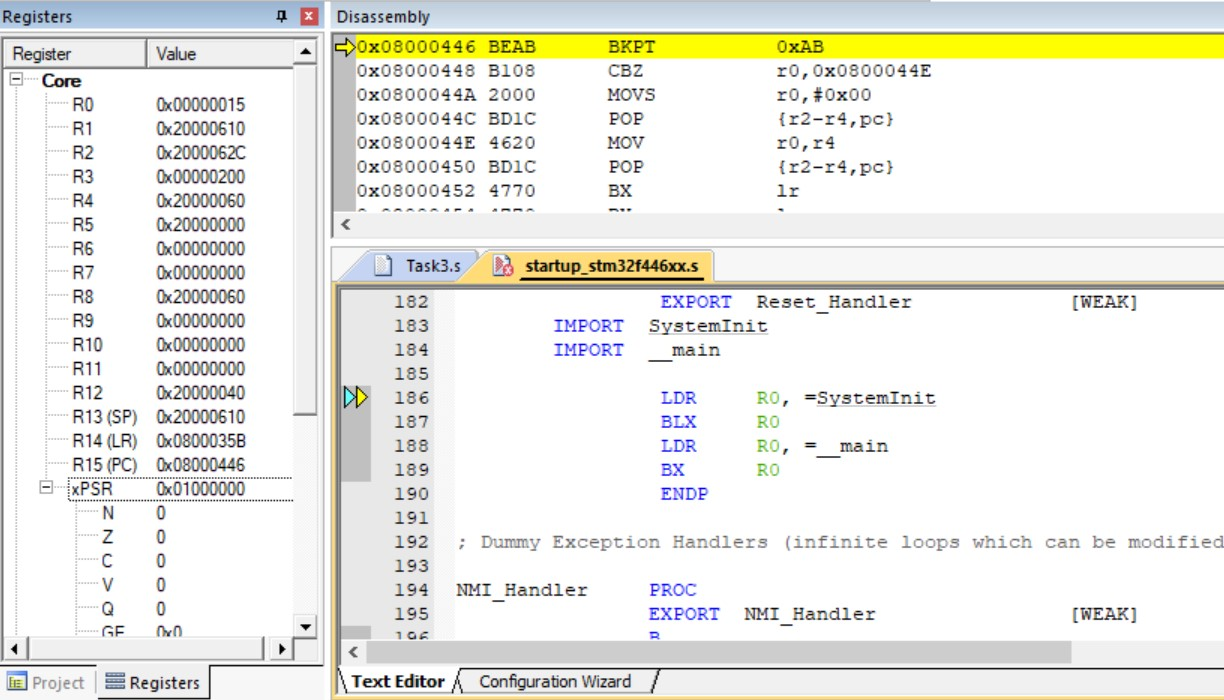
\includegraphics[scale=.7]{images/Task3_1Before1.jpg}
    \caption{After loading the code on the system (Task3\_2\_overflow\_detection)}
    \label{fig:before_task_three_two}
\end{figure}
\FloatBarrier

Here we can see that the registers are loaded with random values as the program is only loaded to the system and not executed yet.
\subsection*{Screenshot of the state of the system after the code has been executed}
\addcontentsline{toc}{subsection}{Screenshot of the state \& status registers of the system after the code has been executed}
\begin{figure}[h!]
    \centering
    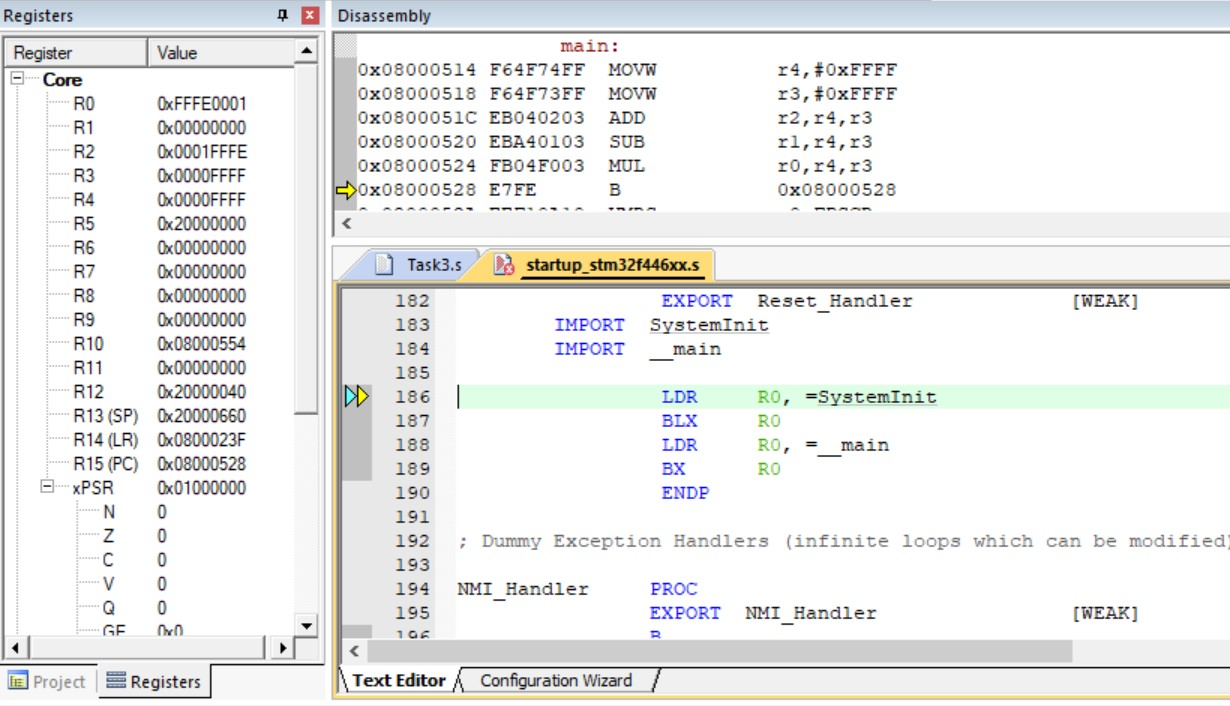
\includegraphics[scale=.7]{images/Task3_1After1.jpg}
    \caption{After executing the code for restricted input on the system (Task3)}
    \label{fig:after_task_three_one_one}
\end{figure}
\FloatBarrier
This is the output for restricted input, we didn't show the status registers in this case because as we're restricting the input to only 16-bit values, no overflow can occur.
\begin{figure}[ht]
    \centering
    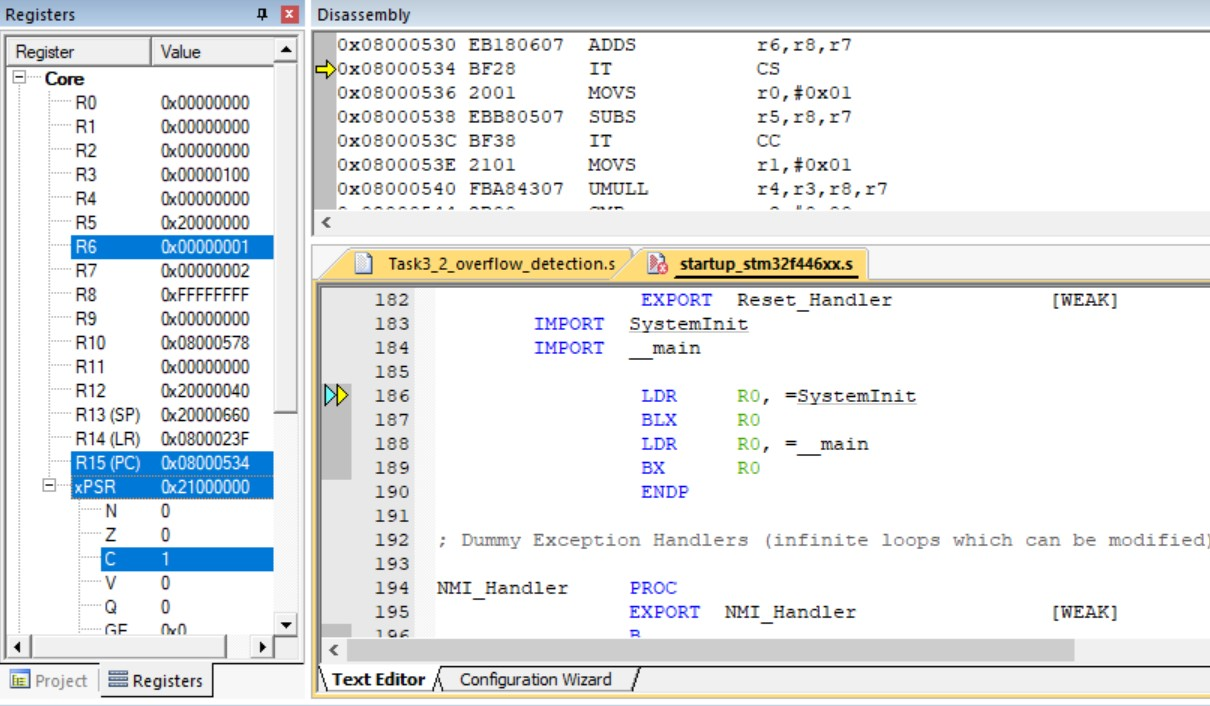
\includegraphics[scale=.7]{images/Task3_2After1.jpg}
    \caption{After executing the code for handling overflow on the system (Task3\_2\_overflow\_detection)}
    \label{fig:after_task_three_two_one}
\end{figure}
\FloatBarrier
This shows the status register or carry flag is set, because overflow occurred. So the value of the register \$r0 remains 1.
\begin{figure}[h!]
    \centering
    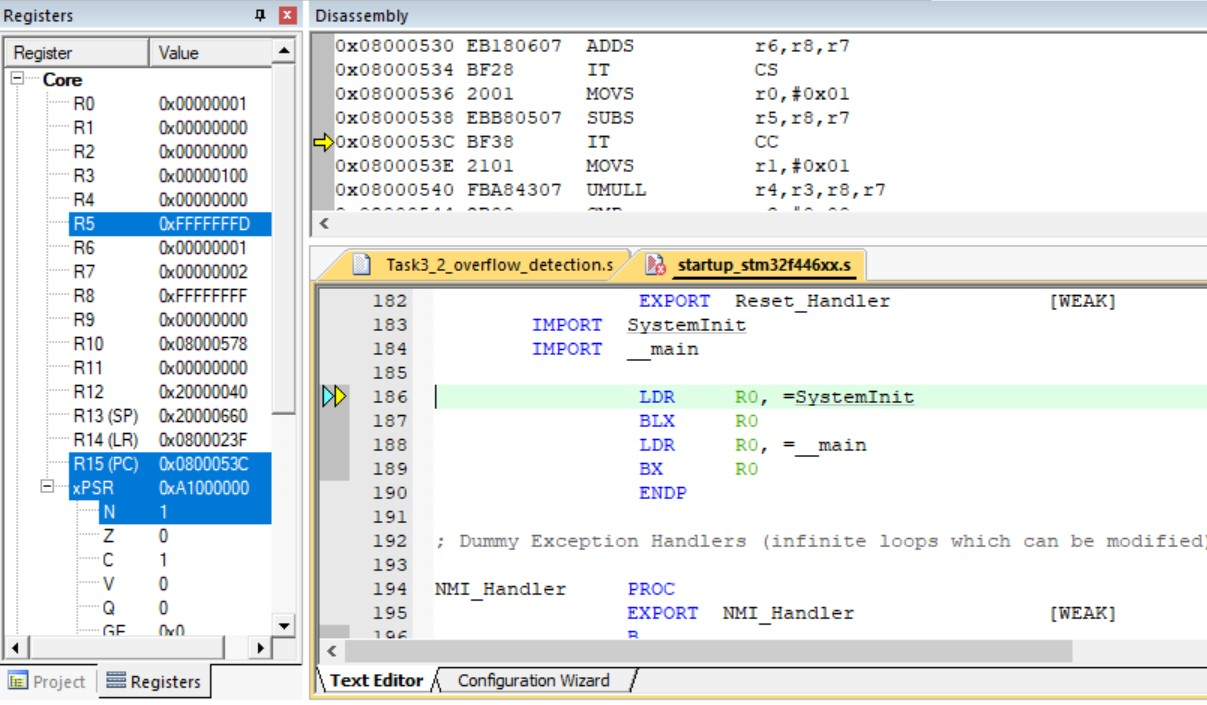
\includegraphics[scale=.7]{images/Task3_2After2.jpg}
    \caption{After executing the code for handling overflow on the system (Task3\_2\_overflow\_detection)}
    \label{fig:after_task_three_two_two}
\end{figure}
\FloatBarrier
This shows the status register carry flag \& negative flag is set, because no overflow occurred in unsigned subtraction (which will always be the case). So the value of the register \$r1 remains 0.
\begin{figure}[ht]
    \centering
    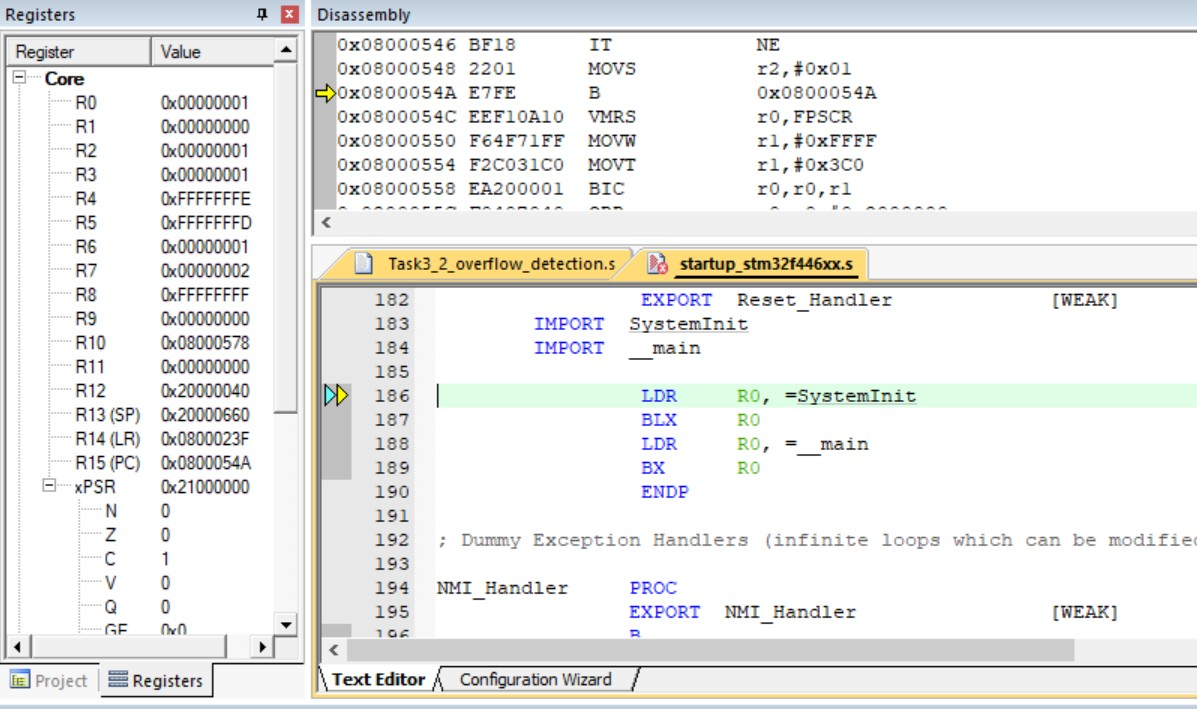
\includegraphics[scale=.7]{images/Task3_2After3.jpg}
    \caption{After executing the code for handling overflow on the system (Task3\_2\_overflow\_detection)}
    \label{fig:after_task_three_two_three}
\end{figure}
\FloatBarrier
This shows that the register \$r2 is set because the multiplication operation resulted in overflow and \verb|$r3 != 0|, so \verb|MOVNE| was executed.\\
This is how we can handle the case of overflow in 32-bit addition, subtraction and multiplication.
\end{document}